\documentclass{beamer}
\usepackage{lmodern}
\usepackage{anyfontsize}
\renewcommand{\normalsize}{\fontsize{14}{16}\selectfont}

\usepackage{tikz}

\usepackage{xcolor} % Cargar el paquete para colores

\usepackage{listings}
\lstset{
    language=Haskell,
    basicstyle=\ttfamily,
    % keywordstyle=\color{blue},
    commentstyle=\color{green!40!black},
    stringstyle=\color{orange},
    showstringspaces=false,
    breaklines=true,
    keywordstyle = [3]{\color{blue}},
    morekeywords = [3]{L},
    keywordstyle = [4]{\color{red}},
    morekeywords = [4]{H}
}

\usetheme{Madrid}
\usecolortheme{default}


%Information to be included in the title page:
\title[Functional Pearl] %optional
{Functional Pearl: \\ Two Can Keep a Secret, If One of Them Uses Haskell}

\subtitle{
}

\author[Joaquin Caporalini] % (optional, for multiple authors)
{
    Alejandro Russo
}

\institute[LCC - FCEIA] % (optional)
{
    Facultad de Ciencias Exactas, Ingeniería y Agrimensura\\Universidad Nacional de Rosario
}

\date[] % (optional)
{\textbf{} \\ Joaquín Caporalini\\Febrero 2025}

\begin{document}

\frame{
    \titlepage
}

% \begin{frame}{Ejemplo con Rectángulos}
%     \begin{tikzpicture}[remember picture, overlay]
%         % Rectángulo con borde rojo y sin relleno en la parte superior izquierda
%         \draw[red, line width=2pt] (0,3) rectangle (3,4);
        
%         % Rectángulo con borde rojo y sin relleno en la parte inferior derecha
%         \draw[red, line width=2pt] (7,-2) rectangle (10,-1);
        
%         % Rectángulo con borde rojo y sin relleno en el centro
%         \draw[red, line width=2pt] (4,1) rectangle (6,2);
%     \end{tikzpicture}
    
%     \centering
%     \textbf{Ejemplo de rectángulos con borde rojo en Beamer}
% \end{frame}

\begin{frame}
    \frametitle{Un encargo para Alice...}
    Construir un gestor de contraseñas simples.\pause Con la función agregada de contraseñas comunes.
    \begin{center}
        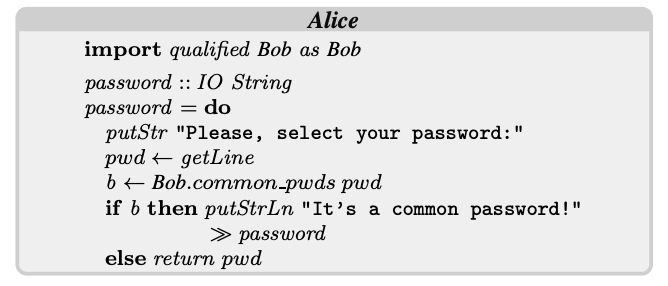
\includegraphics[scale=0.65]{codigo_alice.png}
    \end{center}\pause
    \begin{tikzpicture}[remember picture, overlay]
        % Rectángulo con borde rojo y sin relleno en el centro
        \draw[red, line width=1pt] (3.85,2) rectangle (6.6,1.75);
    \end{tikzpicture}
    El código de Bob:
    \begin{center}
        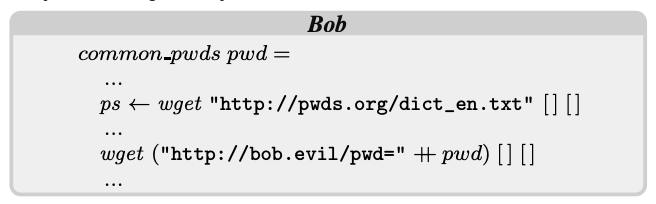
\includegraphics[scale=0.65]{codigo_bob.png}
    \end{center}
\end{frame}

\begin{frame}
    \frametitle{Un encargo para Alice...}
    \textbf{¿Qué debería hacer Alice?}\newline

    Para proteger recursos no alcanza con listas negras (o blancas), sino de asegurar que la información fluye solo hacia los lugares adecuados.\newline
    \pause

    \begin{flushright}
        \it{¿Cómo se logra eso?}
    \end{flushright}

\end{frame}

\begin{frame}
    \frametitle{Mandatory Access Control e Information-Flow Control}
    \begin{itemize}
        \item Asocian datos con etiquetas de seguridad
        para definir su nivel de confidencialidad.
        \item Provienen de la investigación
        \begin{itemize}
            \item MAC: sistemas operativos
            \item IFC: lenguajes de programación
        \end{itemize}
    \end{itemize}
    La propuesta es aprovechar conceptos de lenguajes de programación para implementar mecanismos similares a MAC mediante la creación de una API monádica que protege confidencialidad estáticamente.

\end{frame}

\begin{frame}
    \frametitle{Látice de seguridad}
    \textbf{¿Cómo se etiquetan los datos?}
    Están organizadas en un látice de seguridad.
    \begin{center}
        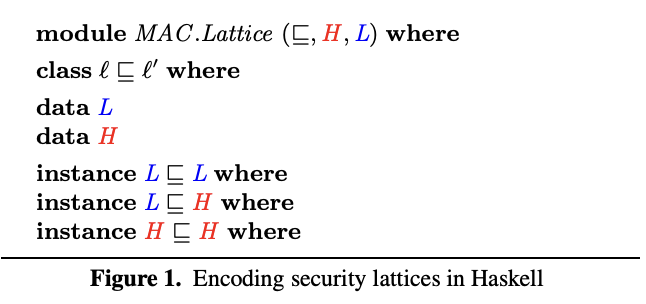
\includegraphics[scale=0.8]{figure1.png}
    \end{center}
    La información no pueda ir de entidades secretas a públicas (no interferencia): $\textcolor{blue}{L} \sqsubseteq \textcolor{red}{H}$ y $\textcolor{red}{H} \not\sqsubseteq \textcolor{blue}{L}$.
\end{frame}

\begin{frame}
    \frametitle{Familia de mónadas MAC}
    Encapsula acciones de IO y restringe su ejecución a situaciones donde la confidencialidad no se ve comprometida.\newline

    Está indexada por una etiqueta de seguridad indicando la sensibilidad de sus resultados monádicos.

    \begin{center}
        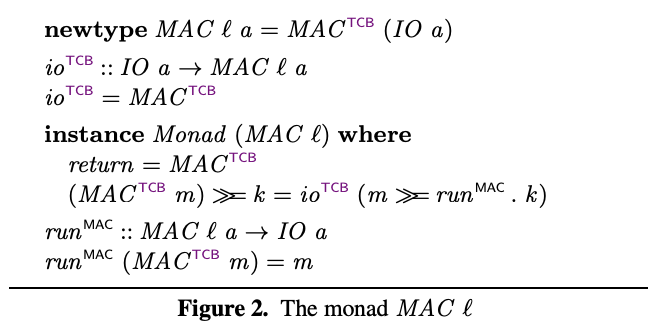
\includegraphics[scale=0.7]{figure2.png}
    \end{center}
\end{frame}

\begin{frame}{Recursos etiquetados}
    
    \begin{center}
        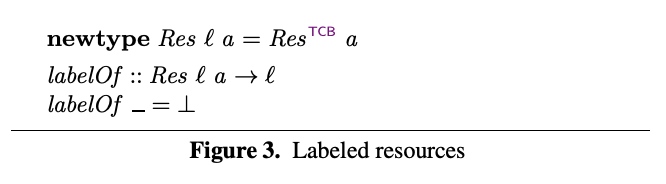
\includegraphics[scale=0.7]{figure3.png}
    \end{center}
    \begin{columns}
        \column{0.5\textwidth}
            \begin{center}
                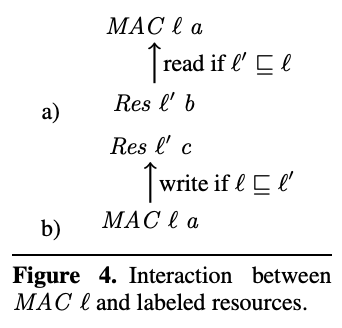
\includegraphics[scale=0.7]{figure4.png}
            \end{center}
        \column{0.5\textwidth}
        Los recursos etiquetados deben tener en cuenta el carácter de los datos, origen y destino. Permite llevar a problema lectura/escritura
    \end{columns}
\end{frame}

\begin{frame}
    \frametitle{Lift de las acciones de IO (Mantener un secreto)}
    Siguiendo los principios de \textit{no read-up} y \textit{no write-down} se extiende la TCB con funciones que elevan las acciones \textit{IO}.

    \begin{center}
        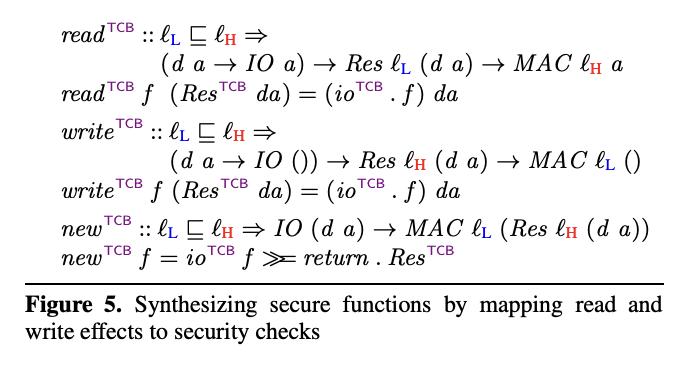
\includegraphics[scale=0.7]{figure5.png}
    \end{center}
\end{frame}

\begin{frame}
    \frametitle{Expresiones etiquetadas}

    Posible etiquetado. Notar el sinónimo de tipo como abreviatura  

    \begin{center}
        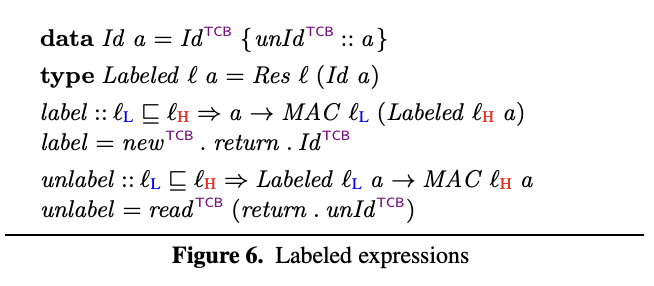
\includegraphics[scale=0.8]{figure6.png}
    \end{center}
\end{frame}

\begin{frame}[fragile]
    \frametitle{Uniendo miembros de la familia}
    Si Bob usase \textit{MAC} su función podría tener el tipo

    \begin{lstlisting}
common_pwds :: Labeled H String -> 
               MAC L (MAC H Bool)
    \end{lstlisting}
    
    En este caso la anidación de computaciones es manejable, pero habrá casos para los que tal vez no, por eso se introduce:

    \begin{center}
        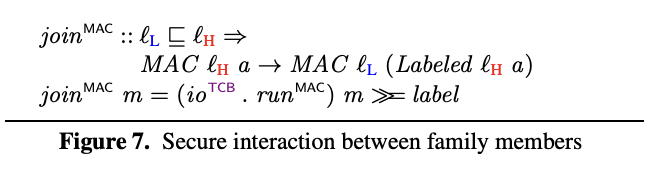
\includegraphics[scale=0.8]{figure7.png}
    \end{center}
\end{frame}

\begin{frame}{Añadiendo referencias (Mutavilidad)}
    \begin{center}
        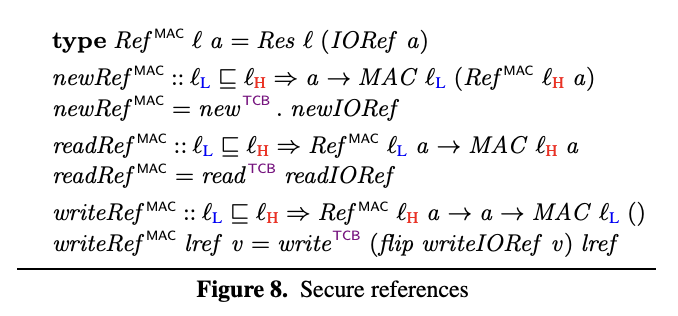
\includegraphics[scale=0.7]{figure8.png}
    \end{center}

    Las funciones se elevan a la mónada $MAC \ l$ envolviéndolas con $new^{TCB}$, $read^{TCB}$ y $write^{TCB}$ respectivamente. \pause

    Estos pasos se generalizan para obtener interfaces seguras de diversos tipos, como veremos más adelante.
\end{frame}

\begin{frame}{Manejo de errores (Excepciones)}
    \begin{center}
        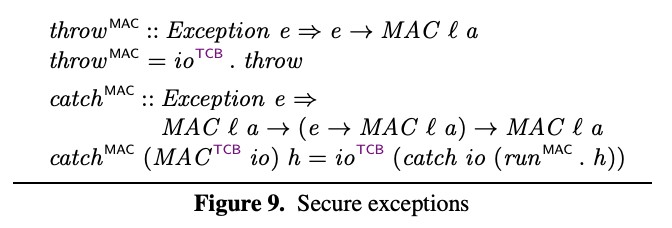
\includegraphics[scale=0.7]{figure9.png}
    \end{center}

    Las excepciones se capturan en el mismo \textbf{tipo} de miembro de la familia donde fueron arrojadas.\newline\pause

    \textbf{Pero, ¿qué pasa con las construcciones con $join^{MAC}$?}
    
    Pueden comprometer la seguridad...
    
    Una acción \textcolor{red}{H} lanzar excepciones y evitar acciones de nivel bajo con la función $join^{MAC}$.
\end{frame}

\begin{frame}{Como lo explotaría un atacante (Bob)}

    \begin{center}
        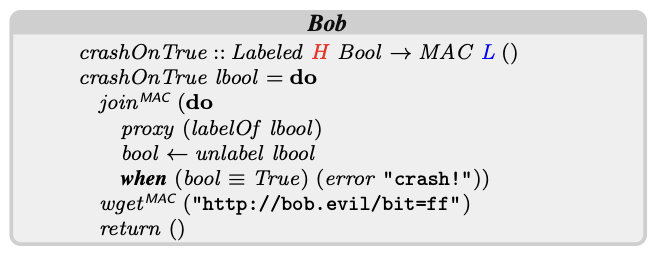
\includegraphics[scale=0.7]{codigo_bob2.png}
    \end{center}

    \begin{center}
        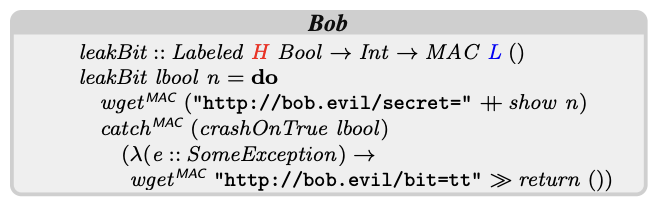
\includegraphics[scale=0.7]{codigo_bob3.png}
    \end{center}
\end{frame}


\begin{frame}{Nuevo $join^{MAC}$}
    Se redefine $join^{MAC}$ de manera tal que la propagación de excepciones entre miembros de la familia quede deshabilitada.

    \begin{center}
        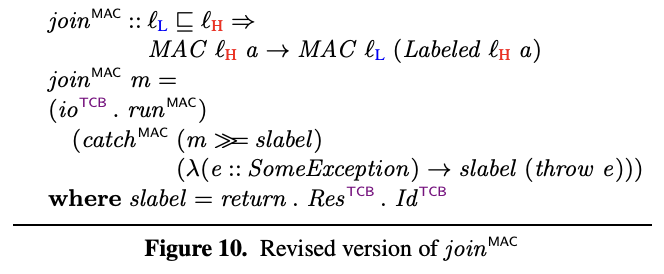
\includegraphics[scale=0.7]{figure10.png}
    \end{center}
\end{frame}

\subsection{El elefante (encubierto) en la habitación}
\begin{frame}{El elefante (encubierto) en la habitación}
    Existe un canal encubierto: la no terminación...\newline

    En un entorno secuencial, la manera más efectiva de explotar un canal encubierto de no-terminación es a través de fuerza bruta, por lo que no hay gran ancho de banda si el universo donde buscar es lo suficientemente grande. \newline
    
    En ese caso se puede omitir el análisis de estos canales encubiertos.

    \vspace{0.5cm}
    \pause
    \begin{flushright}
        \it{¿Pero qué sucede cuando hay concurrencia?}
    \end{flushright}
    
\end{frame}

\begin{frame}{\textit{fork} como primitiva (Concurrencia)}
    Alice añade concurrencia extendiendo la API así:

    \begin{center}
        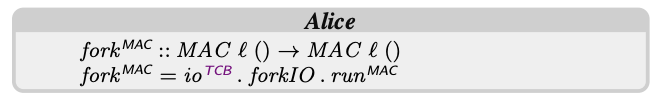
\includegraphics[scale=0.8]{codigo_alice2.png}
    \end{center}

    \textbf{¿Qué ataque puede intentar Bob?}\newline

    Explotar el canal encubierto de la no terminación de programas.
\end{frame}

\begin{frame}{Bob con concurrencia}
    \begin{center}
        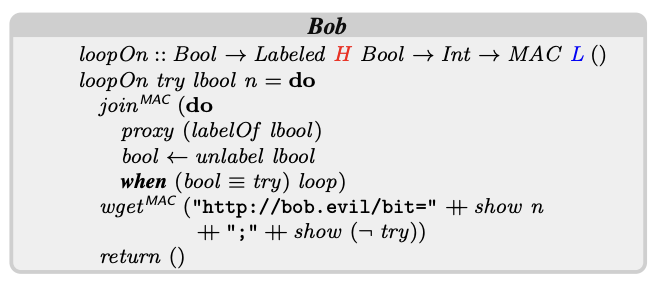
\includegraphics[scale=0.7]{codigo_bob4.png}
    \end{center}

    \begin{center}
        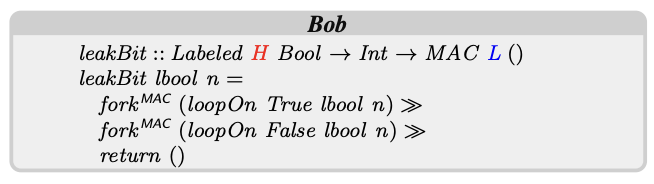
\includegraphics[scale=0.7]{codigo_bob5.png}
    \end{center}
\end{frame}

\begin{frame}{Solución}
    El problema viene de la interacción de $join^{MAC}$ con $fork^{MAC}$.

    Pero, ¡se puede reemplazar a $join^{MAC}$ por $fork^{MAC}$!

    \begin{center}
        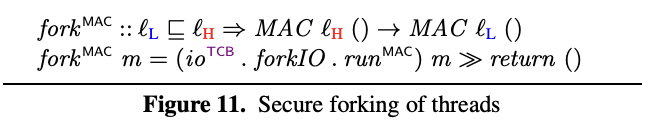
\includegraphics[scale=0.8]{figure11.png}
    \end{center}

    Aunque se haya removido $join^{MAC}$ se pueden combinar computaciones con las referencias seguras introducidas previamente.
\end{frame}

\begin{frame}{MVars (primitivas de sincronización)}
    Se extiende \textbf{MAC} con \textit{MVars} ---una abstracción de sincronización muy utilizada en Haskell--- similar a como se hizo con referencias.
    
    \begin{center}
        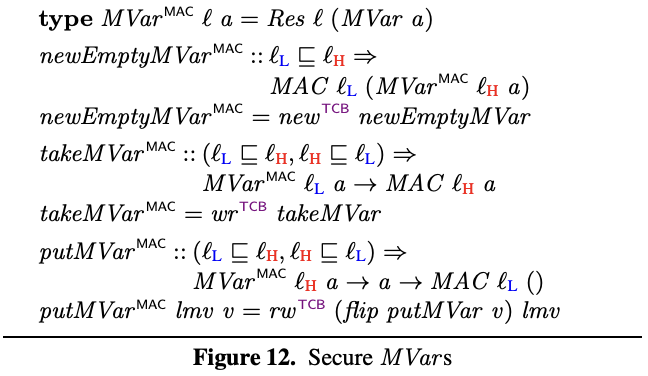
\includegraphics[scale=0.7]{figure12.png}
    \end{center}

    \textbf{TODAS} las acciones provocan el efecto secundario de lecto/escritura.
\end{frame}

\begin{frame}{Comentarios finales}
    \begin{itemize}
        \item<1-> Las abstracciones que provee Haskell y, en general, los lenguajes funcionales, son muy buenas para enfrentarse a los desafíos de seguridad actuales.

        \item<2-> La corrección de \textbf{MAC} depende de la seguridad de tipos y la encapsulación de módulos de Haskell. MAC utiliza Safe Haskell al compilar código no confiable.
        
        \item<3-> La descalcificación intencional no es tratada en este paper sin embargo existen varios enfoques.
        
        \item<4-> Para el ejemplo se uso un etiquetado de dos niveles. Se encontraron formas de usar el sistema de tipos cerrado de GHC para generar extensiones.
    \end{itemize}
\end{frame}

\end{document}